%\documentclass{article} %[twocolumn] 
\documentclass[sagev]{sagej}

%\usepackage{algorithmic}
\usepackage{algorithm}
\usepackage{algorithmicx}
\usepackage{algpseudocode}
\usepackage{booktabs}
\usepackage{array}
\usepackage{graphicx}
\usepackage{amsmath}
\usepackage{amsfonts}
\usepackage{amssymb}
\usepackage{multirow}
\usepackage{url}

\setcounter{secnumdepth}{3} %Gives section numbers for cross referencing
\begin{document}

\runninghead{Wilson et al.}

\title{Robust, value-based sample size determination for clinical trials when nuisance parameters are unknown}

\author{Duncan T. Wilson\affilnum{1}}%,
%Rebecca E. A. Walwyn\affilnum{1}, 
%Richard Hooper\affilnum{2},
%Julia Brown\affilnum{1} and 
%Amanda J. Farrin\affilnum{1}}

\affiliation{\affilnum{1}Leeds Institute of Clinical Trials Research, University of Leeds, Leeds, UK} %\\
%\affilnum{2}Centre for Primary Care \& Public Health, Queen Mary University of London, London, UK}

\corrauth{Duncan T. Wilson, Clinical Trials Research Unit, Leeds Institute of Clinical Trials Research, University of Leeds, Leeds, LS2 9JT, UK}
\email{d.t.wilson@leeds.ac.uk}

\begin{abstract}
% 200 word limit (250 for YSM)

\textbf{Background:} The conventional approach to determining the sample size of a clinical trial is to choose the smallest value such that the power of the trial is above some nominal threshold, often 0.8 or 0.9. This sample size can be highly sensitive to nuisance parameters, such as the variance of a continuous primary outcome. Sample size re-estimation methods allow these parameters to be estimated at an interim analysis to allow the sample size to be adjusted accordingly. However, these methods do not formally account for the associated costs of increased sampling, and as a result can lead to incoherent decisions.

\textbf{Methods:} We present an alternative model for sample size determination which explicitly balances costs and benefits by introducing a value function to be maximised. We explore the implications of the model and argue it provides a better representation of sample size determination in practice than the conventional approach. We show the method is significantly less sensitive than the conventional approach to nuisance parameters, to the point where a fixed design with no interim sample size adjustment can be near-optimal for large regions of the nuisance parameter space. We propose a criterion for choosing an optimal fixed sample size, considering the range of nuisance parameter values for which the value of the fixed design is within a tolerable distance of the value of the best possible design.

\textbf{Results:} We illustrate our approach by applying it to two trial design problems: choosing the accrual and follow-up times for a parallel group trial comparing overall survival, where the median survival time in the control arm is unknown; and choosing the number of clusters in a cluster randomised trial with unknown variance components at both the individual and cluster levels.

\textbf{Conclusion:} Accounting for the costs of sampling when determining the sample size of a clinical trial,  we can find simple, fixed sample size designs which are highly robust to nuisance parameter uncertainty.
\end{abstract}

\keywords{Clinical trials, sample size, power, interim analysis}

\maketitle

\section{Introduction}\label{sec:intro}

\cite{Norman2012} - Sample size calculations: should the emperor's clothes be off the peg or made to measure?

\cite{Edwards1997} - Why "underpowered" trials are not necessarily unethical

\cite{Girling2007} - Sample-size calculations for trials that inform individual treatment decisions: a 'true-choice' approach

\cite{Claxton1999} - The irrelevance of inference: a decision-making approach to the stochastic evaluation of health care technologies

\cite{Grayling2018} - Blinded and unblinded sample size reestimation procedures for stepped-wedge cluster randomized trial

\cite{Altman1980} - Statistics And Ethics In Medical Research: III How Large A Sample?

\cite{DeMartini2010} - Conservative Sample Size Estimation in Nonparametrics



\section{Value-based trial design}

Running example throughout - two sample t-test of means with outcome sd being the nuisance parameter.

The dominant paradigm in clinical trial sample size determination is based on power, the probability of rejecting a null hypothesis conditional on an alternative hypothesis being true. Assuming that the type I error rate is fixed, the two objectives of minimising sample size and maximising power are in conflict. The conventional solution to resolving this is to declare some threshold level of power which must be met, and then find the smallest sample size that satisfies this criteria. As has been previously discussed by others, a major flaw of this approach is that the cost associated with sampling is ignored.

An alternative approach to SSD is to plot the power of the trial as a function of its sample size and to choose the point deemed to best balance cost (i.e. sample size) and benefit (i.e. power). To help describe this decision-making process formally, we can introduce a \emph{value} function $v(n, \beta): \mathbb{N} \times [0,1] \rightarrow \mathbb{R}$ which describes our preferences $\succ$ between all possible pairs of sample size and type II error. Specifically, $v$ is such that
$$
(n, \beta) \succ (n', \beta') \Leftrightarrow v(n, \beta) > v(n', \beta').
$$
Now, if we have a function $f(n)$ that returns the type II error rate obtained for any given choice of sample size (conditional on the remaining aspects of the trial design) then we can define our optimal sample size as
$$
n^* = {\arg\min}_{n \in \mathbb{N}} v(n, f(n)).
$$
What might the value function look like? Consider first a slice of the function with power fixed at some value $\beta_1$, denoted $v_{\beta_1}(n)$. Clearly this will be a strictly decreasing function in $n$, for all $\beta_1$. We propose that it will also be linear, and that the gradient is the same for all $\beta_1$ - that is, the cost of increasing the sample size by some amount $\Delta$ is independent of the starting point $(n_1, \beta_1)$. If a similar linear structure holds for $v_{n_1}(\beta)$, then we have a constant rate of substitution between $n$ and $\beta$. In this case a suitable value function will be of the form 
$$
v(n, \beta) = \beta + \lambda n,
$$
corresponding to linear indifference curves. The optimal sample size can then be obtained by plotting the power curve for the problem at hand and finding the point where the tangent has gradient of $\lambda$ (approximately). For example, consider a two-sample t-test to detect a difference in means of size 1, an outcome standard deviation of $\sigma = 1$, and a value function with $\lambda = 0.025$. The power curve is plotted in Figure \ref{fig:ex1_tangent}, and the optimal sample size is $n = 17$ (giving a power of 0.807). 

\begin{figure}
\centering
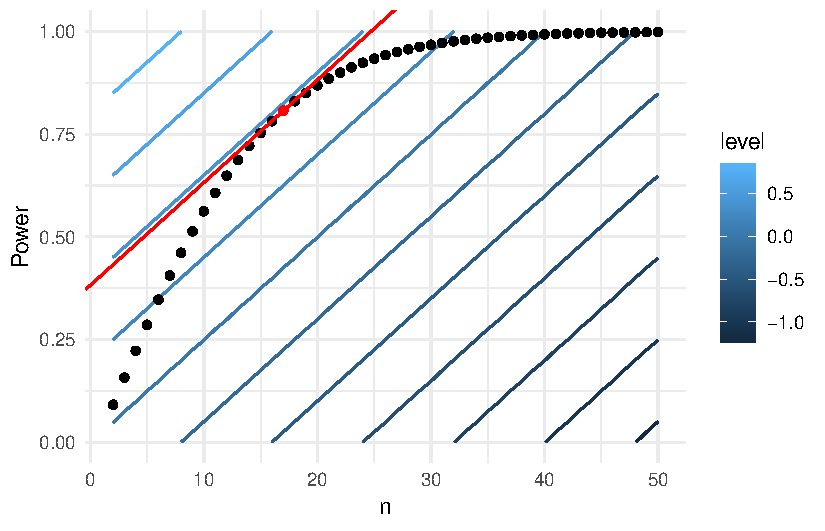
\includegraphics[scale=0.8]{./figures/ex1_tangent}
\caption{.}
\label{fig:ex1_tangent}
\end{figure}

As the figure suggests, if our assumption about the form of the value function holds then we can determine the value of $\lambda$ by simply plotting the power curve and choosing $n$; $\lambda$ is then the gradient of the tangent of the power curve at that point. Is this an accurate representation of our preferences? Do we aggree with its implications? Note that, for example, $\lambda = 0.025$ implies that $(n=0, \beta=0) \sim (n=40, \beta=1)$, and so 40 is the maximum sample size we would ever consider. When it comes to determining $\lambda$, we could use any hypothetical "power" curve and if our assumptions hold we should always choose the sample size that gives the same tangent gradient. For example, consider two other power curves obtained by changing the standard deviation from 1 to 0.7 and 1.3:

\begin{figure}
\centering
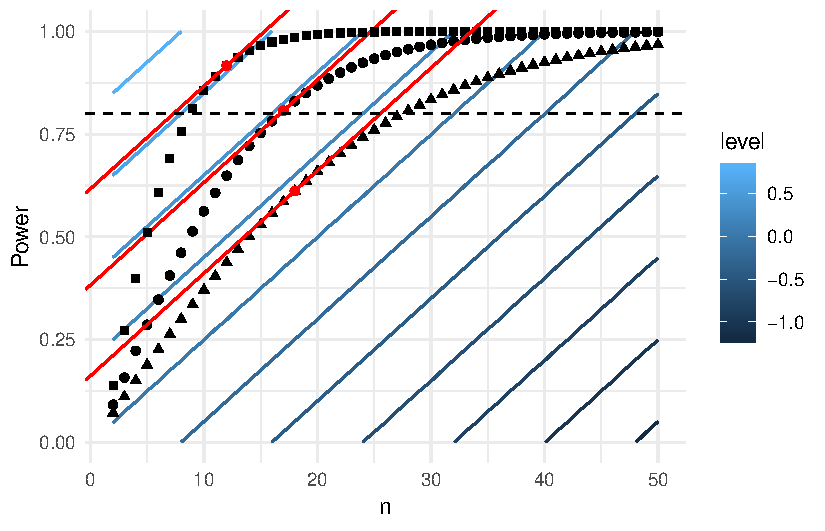
\includegraphics[scale=0.8]{./figures/ex1_3tangents}
\caption{.}
\label{fig:ex1_3tangents}
\end{figure}

On the face of it, this approach seems to be totally inconsistent with the usual method of setting a nominal power to detect our MCID of $\delta = 1$ at (say) 80\%. Under that model, an initial guess of $\sigma = 1$ gives a sample size of $n = 17$, and if we were told our initial estimate of $\sigma = 1$ was incorrect and that actually $\sigma = 1.3$, we should then revise the sample size to $n = 27$ - not $n = 18$ as suggested by our model. But, the common practice of revising the MCID to fit the sample size that is considered `feasible' suggests that the two methods may actually agree. So, we might reason that $n = 27$ is not feasible and unlikely to be funded, and pretend that our MCID is actually $\delta = 1.23$. Then, $n = 18$ will give us 80\% power for this new MCID, but 61\% for the original.

\subsection{Known nuisance parameters}

Normative model is also descriptive, justifying the `sample size samba'.

\subsection{Unknown nuisance parameters}



\section{Examples}

\subsection{Cluster RCT}

\subsection{Survival}

\section{Discussion}

\begin{acks}
Acknowledgements.
\end{acks}

\begin{dci}
The Authors declare that there is no conflict of interest.
\end{dci}

\begin{funding}
This work was supported by the Medical Research Council [grant number xxx].
\end{funding}

\bibliographystyle{SageV}
\bibliography{U:/Literature/Databases/DTWrefs}

\end{document}
